\documentclass[border=3pt]{standalone}
% Preâmbulo compartilhado pelos diagramas TikZ da aula
\usepackage[T1]{fontenc}
\usepackage[utf8]{inputenc}
\usepackage{lmodern}
\usepackage{amsmath}
\usepackage{xcolor}
\usepackage{tikz}
\usetikzlibrary{arrows.meta,angles,quotes,decorations.pathmorphing,calc,
                positioning,shapes.geometric,backgrounds,fit}

% Paleta (mesma dos SVGs originais)
\definecolor{dblue}{HTML}{2A5B8C}
\definecolor{dorange}{HTML}{B3541E}
\definecolor{dgreen}{HTML}{4A7C59}
\definecolor{dred}{HTML}{9C4B4B}
\definecolor{dcream}{HTML}{F4F1EA}
\definecolor{dshade}{HTML}{DDD7C9}

% Estilos comuns (prefixo d... para não colidir com chaves internas do pgf)
\tikzset{
  >={Stealth[length=2mm]},
  dguide/.style={gray!55, dashed, line width=0.4pt},
  daxis/.style={gray!60, line width=0.7pt, ->},
  dbody/.style={fill=black!3, draw=black!80, line width=1pt},
  dacc/.style={draw=dblue, line width=1pt},
  dlbl/.style={black!55, font=\small},
  dsub/.style={black!45, font=\footnotesize},
  dstate/.style={circle, draw=black!80, fill=dcream, line width=1pt,
                 minimum size=17mm, font=\large, inner sep=1pt},
  dobs/.style={circle, draw=black!80, fill=dshade, line width=1pt,
               minimum size=14mm, font=\large, inner sep=1pt},
  dbox/.style={rounded corners=2pt, draw=black!80, fill=dcream, line width=1pt,
               align=center, inner sep=6pt},
  dtrans/.style={->, dblue, line width=1pt},
  dmeas/.style={->, dorange, line width=1pt},
}

\begin{document}
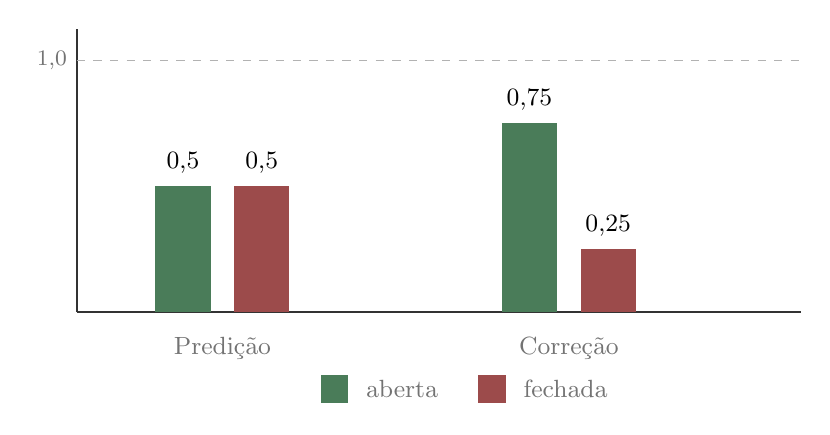
\begin{tikzpicture}[x=1cm,y=1cm]

  \def\H{3.2}  % altura para p = 1,0
  \def\bw{0.7} % largura da barra

  % eixos e linha 1,0
  \draw[black!80, line width=0.8pt] (0,0) -- (9.2,0);
  \draw[black!80, line width=0.8pt] (0,0) -- (0,\H+0.4);
  \draw[black!30, dashed] (0,\H) -- (9.2,\H) node[left, black!55, font=\footnotesize, pos=0] {$1{,}0$};

  % grupo Predição
  \fill[dgreen] (1.0,0) rectangle ++(\bw,{0.5*\H});
  \fill[dred]   (2.0,0) rectangle ++(\bw,{0.5*\H});
  \node[font=\small] at (1.35,{0.5*\H+0.3}) {$0{,}5$};
  \node[font=\small] at (2.35,{0.5*\H+0.3}) {$0{,}5$};
  \node[dlbl] at (1.85,-0.45) {Predição};

  % grupo Correção
  \fill[dgreen] (5.4,0) rectangle ++(\bw,{0.75*\H});
  \fill[dred]   (6.4,0) rectangle ++(\bw,{0.25*\H});
  \node[font=\small] at (5.75,{0.75*\H+0.3}) {$0{,}75$};
  \node[font=\small] at (6.75,{0.25*\H+0.3}) {$0{,}25$};
  \node[dlbl] at (6.25,-0.45) {Correção};

  % legenda
  \fill[dgreen] (3.1,-1.15) rectangle ++(0.35,0.35);
  \node[dlbl, anchor=west] at (3.55,-0.97) {aberta};
  \fill[dred]   (5.1,-1.15) rectangle ++(0.35,0.35);
  \node[dlbl, anchor=west] at (5.55,-0.97) {fechada};

\end{tikzpicture}
\end{document}
